\documentclass[../PHYS306Notes.tex]{subfiles}

\begin{document}
\section{Lecture 20}
\subsection{Lecture Notes - Free Rotation of Spinning Top \& Euler Angles}
\subsubsection{Euler Equations Review}
\begin{center}
    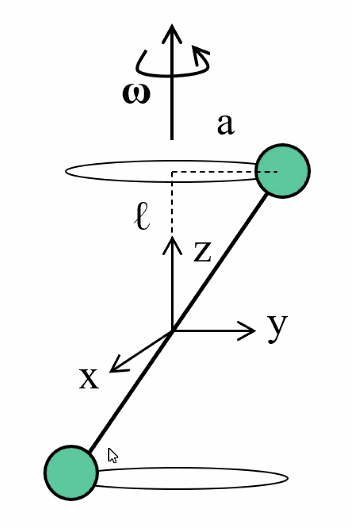
\includegraphics[scale=0.5]{Lecture-20/l20-img1.png}
\end{center}
A rotating dumbbell consists of two masses $m$ which move in circles at a $z$ displacement $l$ and $-l$, joined by a massless rod. The angular velocity vector is $\bm{\omega} = \omega\zhat$. Consider the body frame where the positions of the masses are $(0, a, l)$ and $(0, -a, -l)$. What are the principle axes of inertia?
\begin{center}
    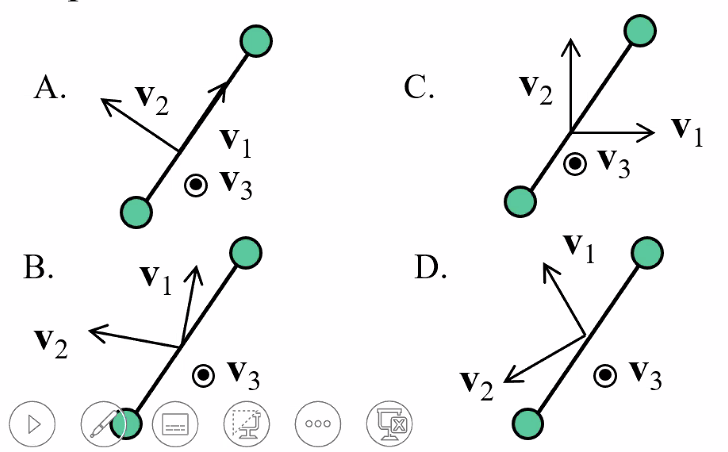
\includegraphics[scale=0.5]{Lecture-20/l20-img2.png}
\end{center}
\begin{s}
A). The principle axes of inertia are aligned with the symmetries of the body. If there is a symmetry axes, we can expect this to correspond to a principle axis.
\end{s}
\begin{center}
    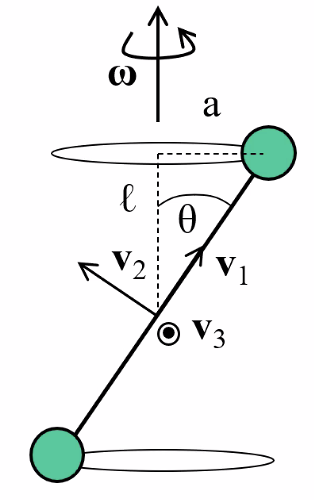
\includegraphics[scale=0.5]{Lecture-20/l20-img3.png}
\end{center}
Followup: What is the components of the angular velocity vector in this frame? (where $\theta$ is the angle formed by the z-axis/rotation axis and the mass?)
\begin{s}
$\bm{\omega} = \m{\omega\cos\theta \\ \omega\sin\theta \\ 0}$ by trigonometry. 
\end{s}
Consider the body frame aligned with the principle axes of inertia (as sketched). What are Euler's equations in this frame?
\begin{s}
We first recall the three moments of inertia:
\[\lambda_1 = 0\]
\[\lambda_2 = 2m(a^2 + l^2)\]
\[\lambda_3 = 2m(a^2 + l^2)\]
We also recall the Euler equations:
\[\Gamma_1 = \lambda_1\dot{\omega}_1 - (\lambda_2 - \lambda_3)\omega_2\omega_3\]
\[\Gamma_2 = \lambda_2\dot{\omega}_2 - (\lambda_3 - \lambda_1)\omega_1\omega_3\]
\[\Gamma_3 = \lambda_3\dot{\omega}_3 - (\lambda_1 - \lambda_2)\omega_1\omega_2\]
In this case, we have that $\omega_3$ along $\v{v}_3$ is zero (from the previous problem) and that the time derivatives of all of the $\omega_i$s are zero (as the dumbell rotates at constant velocity. From this we get:
\[\Gamma_1 = 0\]
\[\Gamma_2 = 0\]
\[\Gamma3 = 2m(a^2 + l^2)\omega^2\sin\theta\cos\theta\]
\end{s}
Cosnider the body frame aligned with the principle axes of inertia.  In this frame, the torque is constant in the 3 directions (out of the page). How can you describe the torque in the space frame?
\begin{s}
Since $\v{L}$ is rotating and $\bm{\Gamma}$ is perpendicular to this and rotating with it (in the lab frame), we therefore have that $\abs{\bm{\Gamma}}$ is constant and it is rotating about the z axis.
\end{s}
What is the angular momentum in the body frame?
\begin{s}
$\v{L} = \II\bm{\omega}$, and since $\II$ is diagonal in the body frame, we have:
\[\v{L} = \II\bm{\omega} = \m{0 & 0 & 0 \\ 0 & 2m(a^2+l^2) & 0 \\ 0 & 0 & 2m(a^2 + l^2)}\m{\omega\cos\theta \\ \omega\sin\theta \\ 0} = \m{0 \\ 2m(a^2+l^2)\omega\sin\theta \\ 0}\]
\end{s}

\subsubsection{Free Rotation of symmetric top}
Here, we study the motion of a symmetric top. This means that $\lambda_1 = \lambda_2$. In addition, no torque, so $\bm{\Gamma} = \v{0}$. Writing down the Euler equations (where the LHS will be zero), we then have:
\[0 = \lambda_1\dot{\omega}_1 - (\lambda_2 - \lambda_3)\omega_2\omega_3\]
\[0 = \lambda_2\dot{\omega}_2 - (\lambda_3 - \lambda_1)\omega_1\omega_3\]
\[0 = \lambda_3\dot{\omega}_3 - (\lambda_1 - \lambda_2)\omega_1\omega_2\]
Since $\lambda_1 - \lambda_2 = 0$, we therefore find that $\dot{\omega}_3 = 0$ and hence $\omega_3$ is constant (as lines up with our experience. Writing the other equations down (making the substitution that $\lambda_2 = \lambda_1$, we have:
\[\dot{\omega}_1 = \frac{\lambda_1 - \lambda_3}{\lambda_1}\omega_2\omega_3\]
\[\dot{\omega}_2 = -\frac{\lambda_1 - \lambda_3}{\lambda_1}\omega_1\omega_3\]
Let us define $\Omega_b = \frac{\lambda_1 - \lambda_3}{\lambda_1}\omega_3$, then we have:
\[\dot{\omega}_1 = \Omega_b\omega_2\]
\[\dot{\omega}_2 = -\Omega_b\omega1\]
Let us add $i$ times the second equation to the first equation. Then, define $\eta = \omega_1 + i\omega_2$. We then have:
\[\dot{\omega}_1 + i\dot{\omega}_2 = \dot{\eta} = \Omega_b(\omega_2 - i\omega_1) = -i\Omega_b\eta\]
This has a complex exponential solution:
\[\eta(t) = \eta_0\exp(-i\Omega_b t)\]
Suppose $\eta_0 = \omega_0$. then:
\[\eta(t) = \omega_0\exp(-i\Omega_b t)\]
Takign the real and imaginary parts to recover $\omega_1$ and $\omega_2$, we get:
\[\bm{\omega} = \m{\omega_0\cos(\Omega_b t) \\ -\omega_0\sin(\Omega_b t) \\ \omega_3}\]
From which we can see tha the free top undergoes precession. We can check that $\dot{bm{\omega}} = \bm{\Omega}_b \times \bm{\omega}$ which would indeed correspond to rotation. We note that $\abs{\bm{\omega}}$ is a constant here. Visually, we could think of these as follows:
\begin{center}
    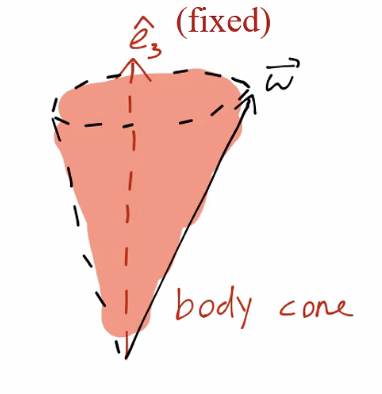
\includegraphics[scale=0.5]{Lecture-20/l20-img4.png}
    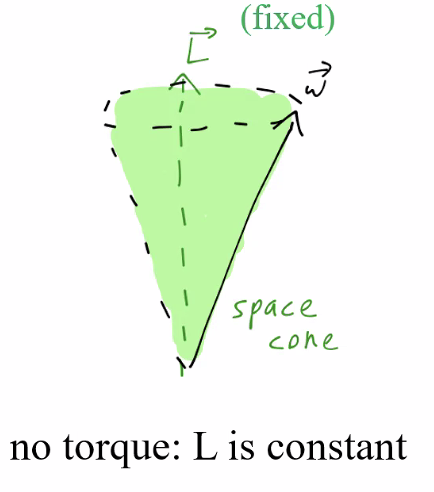
\includegraphics[scale=0.5]{Lecture-20/l20-img5.png}
    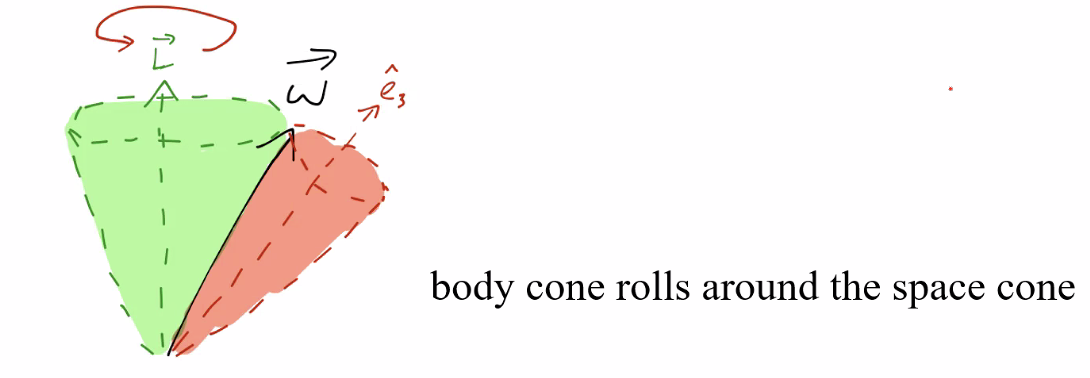
\includegraphics[scale=0.5]{Lecture-20/l20-img6.png}
\end{center}

\subsubsection{Rotation Matrices}
We need to establish a more systematic way to go from body to lab frame (i.e. rotating the coordinate system). 
\begin{center}
    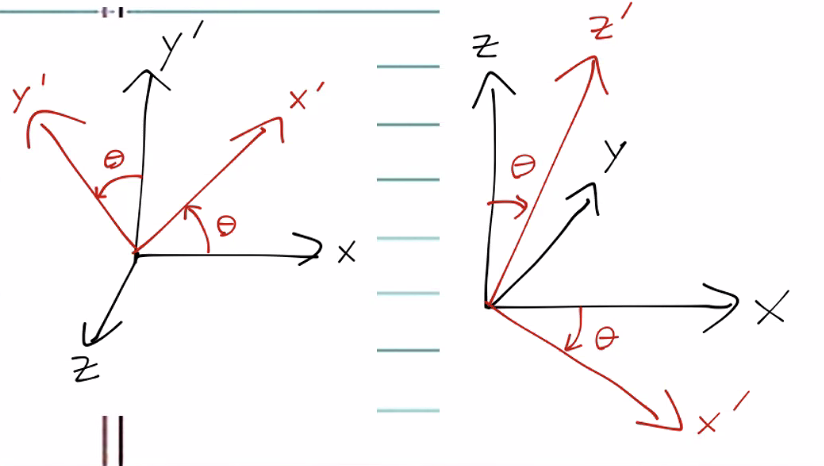
\includegraphics[scale=0.5]{Lecture-20/l20-img7.png}
\end{center}
These rotations are performed through rotation matrices. The first picture is a rotation around the z axis. The matrix that does this is
\[R_z = \m{\cos\theta & \sin\theta & 0 \\ -\sin\theta & \cos\theta & 0 \\ 0 & 0 & 1}\]
The second picture is a rotation around the y axis. The matrix that does this is:
\[R_y = \m{\cos\theta & 0 & -\sin\theta \\ 0 & 1 & 0 \\ \sin\theta & 0 & \cos\theta}\]
Where the minus sign is switched in order to preserve the handedness of the coordinate system. X is the same, with:
\[R_x = \m{1 & 0 & 0 \\ 0 & \cos\theta & \sin\theta \\ 0 & -\sin\theta & \cos\theta}\]
In general, to go from one coordinate system to another, we can decompose the rotations into rotations about x, y, and z. But note that the \textbf{order matters}! This brings us to discussion of Euler angles.

\subsubsection{Euler Angles}
The Euler angles gives us a convention for the order of rotations.
\begin{center}
    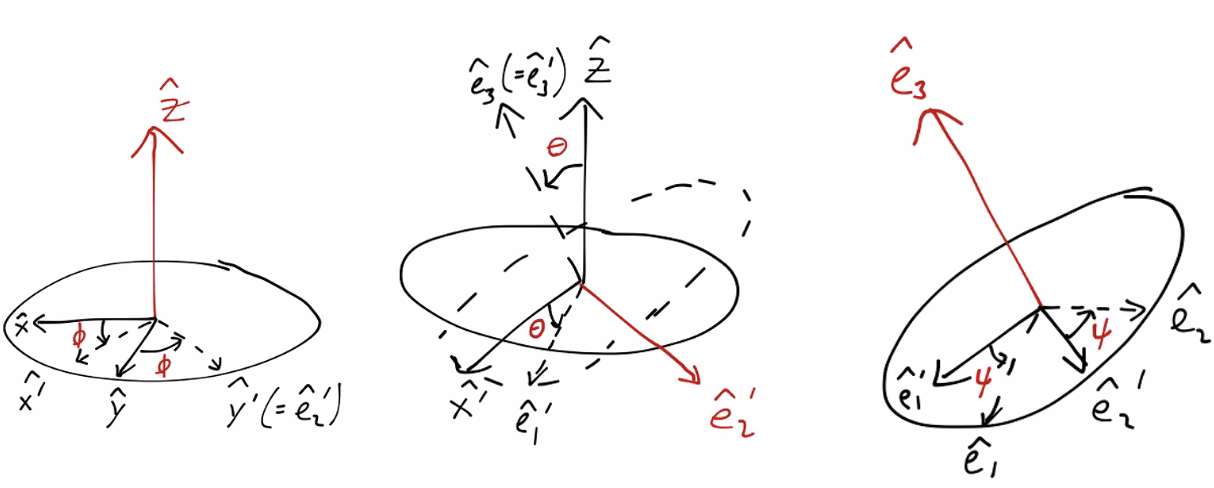
\includegraphics[scale=0.5]{Lecture-20/l20-img8.png}
\end{center}
\begin{enumerate}[1.]
\item First, we rotate around the z-axis by $\phi$.
\item Next, we rotate around the \textbf{new} y axis by $\theta$
\item Finally, we rotate around the \textbf{new} z-axis by $\psi$.
\end{enumerate}
Next day: A general Lagrangian for rigid systems, and then applying this to a spinning top with Torque applied to it. Then, we get into Hamiltonian mechanics!
\end{document}